\documentclass[1p]{elsarticle_modified}
%\bibliographystyle{elsarticle-num}

%\usepackage[colorlinks]{hyperref}
%\usepackage{abbrmath_seonhwa} %\Abb, \Ascr, \Acal ,\Abf, \Afrak
\usepackage{amsfonts}
\usepackage{amssymb}
\usepackage{amsmath}
\usepackage{amsthm}
\usepackage{scalefnt}
\usepackage{amsbsy}
\usepackage{kotex}
\usepackage{caption}
\usepackage{subfig}
\usepackage{color}
\usepackage{graphicx}
\usepackage{xcolor} %% white, black, red, green, blue, cyan, magenta, yellow
\usepackage{float}
\usepackage{setspace}
\usepackage{hyperref}

\usepackage{tikz}
\usetikzlibrary{arrows}

\usepackage{multirow}
\usepackage{array} % fixed length table
\usepackage{hhline}

%%%%%%%%%%%%%%%%%%%%%
\makeatletter
\renewcommand*\env@matrix[1][\arraystretch]{%
	\edef\arraystretch{#1}%
	\hskip -\arraycolsep
	\let\@ifnextchar\new@ifnextchar
	\array{*\c@MaxMatrixCols c}}
\makeatother %https://tex.stackexchange.com/questions/14071/how-can-i-increase-the-line-spacing-in-a-matrix
%%%%%%%%%%%%%%%

\usepackage[normalem]{ulem}

\newcommand{\msout}[1]{\ifmmode\text{\sout{\ensuremath{#1}}}\else\sout{#1}\fi}
%SOURCE: \msout is \stkout macro in https://tex.stackexchange.com/questions/20609/strikeout-in-math-mode

\newcommand{\cancel}[1]{
	\ifmmode
	{\color{red}\msout{#1}}
	\else
	{\color{red}\sout{#1}}
	\fi
}

\newcommand{\add}[1]{
	{\color{blue}\uwave{#1}}
}

\newcommand{\replace}[2]{
	\ifmmode
	{\color{red}\msout{#1}}{\color{blue}\uwave{#2}}
	\else
	{\color{red}\sout{#1}}{\color{blue}\uwave{#2}}
	\fi
}

\newcommand{\Sol}{\mathcal{S}} %segment
\newcommand{\D}{D} %diagram
\newcommand{\A}{\mathcal{A}} %arc


%%%%%%%%%%%%%%%%%%%%%%%%%%%%%5 test

\def\sl{\operatorname{\textup{SL}}(2,\Cbb)}
\def\psl{\operatorname{\textup{PSL}}(2,\Cbb)}
\def\quan{\mkern 1mu \triangleright \mkern 1mu}

\theoremstyle{definition}
\newtheorem{thm}{Theorem}[section]
\newtheorem{prop}[thm]{Proposition}
\newtheorem{lem}[thm]{Lemma}
\newtheorem{ques}[thm]{Question}
\newtheorem{cor}[thm]{Corollary}
\newtheorem{defn}[thm]{Definition}
\newtheorem{exam}[thm]{Example}
\newtheorem{rmk}[thm]{Remark}
\newtheorem{alg}[thm]{Algorithm}

\newcommand{\I}{\sqrt{-1}}
\begin{document}

%\begin{frontmatter}
%
%\title{Boundary parabolic representations of knots up to 8 crossings}
%
%%% Group authors per affiliation:
%\author{Yunhi Cho} 
%\address{Department of Mathematics, University of Seoul, Seoul, Korea}
%\ead{yhcho@uos.ac.kr}
%
%
%\author{Seonhwa Kim} %\fnref{s_kim}}
%\address{Center for Geometry and Physics, Institute for Basic Science, Pohang, 37673, Korea}
%\ead{ryeona17@ibs.re.kr}
%
%\author{Hyuk Kim}
%\address{Department of Mathematical Sciences, Seoul National University, Seoul 08826, Korea}
%\ead{hyukkim@snu.ac.kr}
%
%\author{Seokbeom Yoon}
%\address{Department of Mathematical Sciences, Seoul National University, Seoul, 08826,  Korea}
%\ead{sbyoon15@snu.ac.kr}
%
%\begin{abstract}
%We find all boundary parabolic representation of knots up to 8 crossings.
%
%\end{abstract}
%\begin{keyword}
%    \MSC[2010] 57M25 
%\end{keyword}
%
%\end{frontmatter}

%\linenumbers
%\tableofcontents
%
\newcommand\colored[1]{\textcolor{white}{\rule[-0.35ex]{0.8em}{1.4ex}}\kern-0.8em\color{red} #1}%
%\newcommand\colored[1]{\textcolor{white}{ #1}\kern-2.17ex	\textcolor{white}{ #1}\kern-1.81ex	\textcolor{white}{ #1}\kern-2.15ex\color{red}#1	}

{\Large $\underline{12n_{0074}~(K12n_{0074})}$}

\setlength{\tabcolsep}{10pt}
\renewcommand{\arraystretch}{1.6}
\vspace{1cm}\begin{tabular}{m{100pt}>{\centering\arraybackslash}m{274pt}}
\multirow{5}{120pt}{
	\centering
	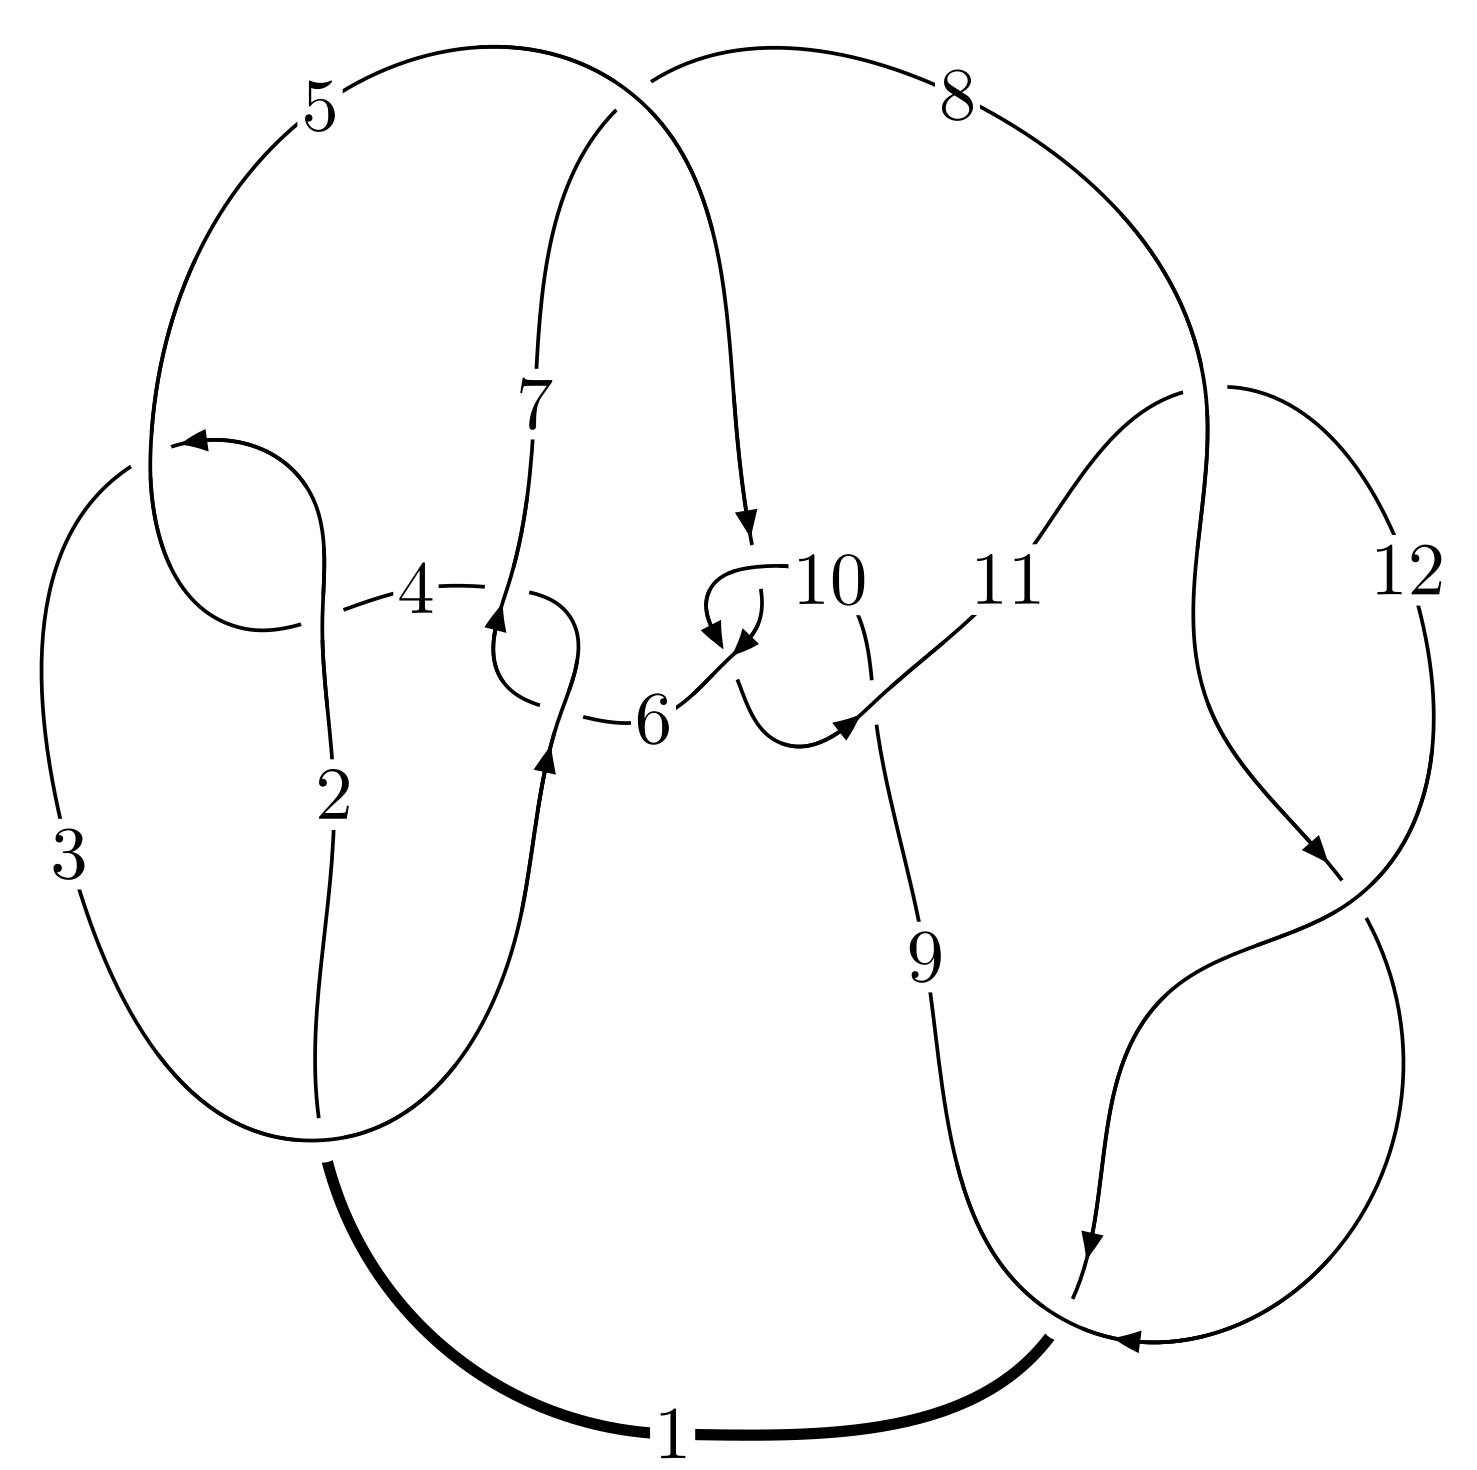
\includegraphics[width=112pt]{../../../GIT/diagram.site/Diagrams/png/2163_12n_0074.png}\\
\ \ \ A knot diagram\footnotemark}&
\allowdisplaybreaks
\textbf{Linearized knot diagam} \\
\cline{2-2}
 &
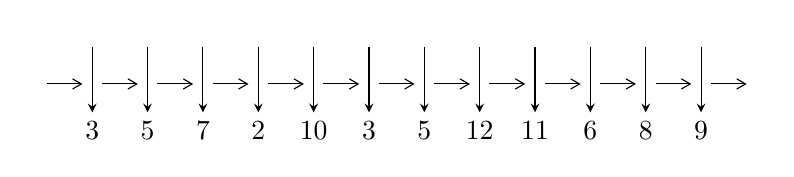
\begin{tikzpicture}[x=20pt, y=17pt]
	% nodes
	\node (C0) at (0, 0) {};
	\node (C1) at (1, 0) {};
	\node (C1U) at (1, +1) {};
	\node (C1D) at (1, -1) {3};

	\node (C2) at (2, 0) {};
	\node (C2U) at (2, +1) {};
	\node (C2D) at (2, -1) {5};

	\node (C3) at (3, 0) {};
	\node (C3U) at (3, +1) {};
	\node (C3D) at (3, -1) {7};

	\node (C4) at (4, 0) {};
	\node (C4U) at (4, +1) {};
	\node (C4D) at (4, -1) {2};

	\node (C5) at (5, 0) {};
	\node (C5U) at (5, +1) {};
	\node (C5D) at (5, -1) {10};

	\node (C6) at (6, 0) {};
	\node (C6U) at (6, +1) {};
	\node (C6D) at (6, -1) {3};

	\node (C7) at (7, 0) {};
	\node (C7U) at (7, +1) {};
	\node (C7D) at (7, -1) {5};

	\node (C8) at (8, 0) {};
	\node (C8U) at (8, +1) {};
	\node (C8D) at (8, -1) {12};

	\node (C9) at (9, 0) {};
	\node (C9U) at (9, +1) {};
	\node (C9D) at (9, -1) {11};

	\node (C10) at (10, 0) {};
	\node (C10U) at (10, +1) {};
	\node (C10D) at (10, -1) {6};

	\node (C11) at (11, 0) {};
	\node (C11U) at (11, +1) {};
	\node (C11D) at (11, -1) {8};

	\node (C12) at (12, 0) {};
	\node (C12U) at (12, +1) {};
	\node (C12D) at (12, -1) {9};
	\node (C13) at (13, 0) {};

	% arrows
	\draw[->,>={angle 60}]
	(C0) edge (C1) (C1) edge (C2) (C2) edge (C3) (C3) edge (C4) (C4) edge (C5) (C5) edge (C6) (C6) edge (C7) (C7) edge (C8) (C8) edge (C9) (C9) edge (C10) (C10) edge (C11) (C11) edge (C12) (C12) edge (C13) ;	\draw[->,>=stealth]
	(C1U) edge (C1D) (C2U) edge (C2D) (C3U) edge (C3D) (C4U) edge (C4D) (C5U) edge (C5D) (C6U) edge (C6D) (C7U) edge (C7D) (C8U) edge (C8D) (C9U) edge (C9D) (C10U) edge (C10D) (C11U) edge (C11D) (C12U) edge (C12D) ;
	\end{tikzpicture} \\
\hhline{~~} \\& 
\textbf{Solving Sequence} \\ \cline{2-2} 
 &
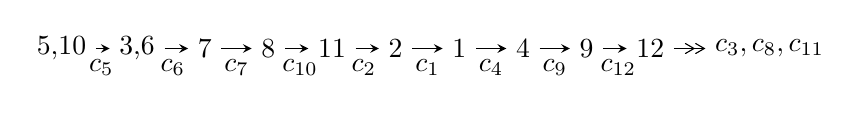
\begin{tikzpicture}[x=23pt, y=7pt]
	% node
	\node (A0) at (-1/8, 0) {5,10};
	\node (A1) at (17/16, 0) {3,6};
	\node (A2) at (17/8, 0) {7};
	\node (A3) at (25/8, 0) {8};
	\node (A4) at (33/8, 0) {11};
	\node (A5) at (41/8, 0) {2};
	\node (A6) at (49/8, 0) {1};
	\node (A7) at (57/8, 0) {4};
	\node (A8) at (65/8, 0) {9};
	\node (A9) at (73/8, 0) {12};
	\node (C1) at (1/2, -1) {$c_{5}$};
	\node (C2) at (13/8, -1) {$c_{6}$};
	\node (C3) at (21/8, -1) {$c_{7}$};
	\node (C4) at (29/8, -1) {$c_{10}$};
	\node (C5) at (37/8, -1) {$c_{2}$};
	\node (C6) at (45/8, -1) {$c_{1}$};
	\node (C7) at (53/8, -1) {$c_{4}$};
	\node (C8) at (61/8, -1) {$c_{9}$};
	\node (C9) at (69/8, -1) {$c_{12}$};
	\node (A10) at (11, 0) {$c_{3},c_{8},c_{11}$};

	% edge
	\draw[->,>=stealth]	
	(A0) edge (A1) (A1) edge (A2) (A2) edge (A3) (A3) edge (A4) (A4) edge (A5) (A5) edge (A6) (A6) edge (A7) (A7) edge (A8) (A8) edge (A9) ;
	\draw[->>,>={angle 60}]	
	(A9) edge (A10);
\end{tikzpicture} \\ 

\end{tabular} \\

\footnotetext{
The image of knot diagram is generated by the software ``\textbf{Draw programme}" developed by Andrew Bartholomew(\url{http://www.layer8.co.uk/maths/draw/index.htm\#Running-draw}), where we modified some parts for our purpose(\url{https://github.com/CATsTAILs/LinksPainter}).
}\phantom \\ \newline 
\centering \textbf{Ideals for irreducible components\footnotemark of $X_{\text{par}}$} 
 
\begin{align*}
I^u_{1}&=\langle 
-1.18522\times10^{30} u^{33}+1.61395\times10^{30} u^{32}+\cdots+1.16116\times10^{30} b+7.98061\times10^{30},\\
\phantom{I^u_{1}}&\phantom{= \langle  }-5.04287\times10^{30} u^{33}+7.56763\times10^{30} u^{32}+\cdots+2.32232\times10^{30} a+4.15748\times10^{31},\;u^{34}-2 u^{33}+\cdots-4 u+4\rangle \\
I^u_{2}&=\langle 
b+1,\;2 u^7- u^6-3 u^5+3 u^4+4 u^3-3 u^2+a-2 u+4,\;u^8- u^7- u^6+2 u^5+u^4-2 u^3+2 u-1\rangle \\
\\
I^v_{1}&=\langle 
a,\;b- v-2,\;v^2+3 v+1\rangle \\
\end{align*}
\raggedright * 3 irreducible components of $\dim_{\mathbb{C}}=0$, with total 44 representations.\\
\footnotetext{All coefficients of polynomials are rational numbers. But the coefficients are sometimes approximated in decimal forms when there is not enough margin.}
\newpage
\renewcommand{\arraystretch}{1}
\centering \section*{I. $I^u_{1}= \langle -1.19\times10^{30} u^{33}+1.61\times10^{30} u^{32}+\cdots+1.16\times10^{30} b+7.98\times10^{30},\;-5.04\times10^{30} u^{33}+7.57\times10^{30} u^{32}+\cdots+2.32\times10^{30} a+4.16\times10^{31},\;u^{34}-2 u^{33}+\cdots-4 u+4 \rangle$}
\flushleft \textbf{(i) Arc colorings}\\
\begin{tabular}{m{7pt} m{180pt} m{7pt} m{180pt} }
\flushright $a_{5}=$&$\begin{pmatrix}1\\0\end{pmatrix}$ \\
\flushright $a_{10}=$&$\begin{pmatrix}0\\u\end{pmatrix}$ \\
\flushright $a_{3}=$&$\begin{pmatrix}2.17148 u^{33}-3.25864 u^{32}+\cdots-25.8226 u-17.9022\\1.02072 u^{33}-1.38995 u^{32}+\cdots-3.99583 u-6.87295\end{pmatrix}$ \\
\flushright $a_{6}=$&$\begin{pmatrix}1\\u^2\end{pmatrix}$ \\
\flushright $a_{7}=$&$\begin{pmatrix}0.786569 u^{33}-1.29705 u^{32}+\cdots-10.0199 u-7.25363\\1.01950 u^{33}-1.41535 u^{32}+\cdots-4.86444 u-6.48780\end{pmatrix}$ \\
\flushright $a_{8}=$&$\begin{pmatrix}-0.232929 u^{33}+0.118296 u^{32}+\cdots-5.15543 u-0.765831\\1.01950 u^{33}-1.41535 u^{32}+\cdots-4.86444 u-6.48780\end{pmatrix}$ \\
\flushright $a_{11}=$&$\begin{pmatrix}- u\\- u^3+u\end{pmatrix}$ \\
\flushright $a_{2}=$&$\begin{pmatrix}3.19220 u^{33}-4.64859 u^{32}+\cdots-29.8184 u-24.7752\\1.02072 u^{33}-1.38995 u^{32}+\cdots-3.99583 u-6.87295\end{pmatrix}$ \\
\flushright $a_{1}=$&$\begin{pmatrix}0.786569 u^{33}-1.29705 u^{32}+\cdots-10.0199 u-7.25363\\-0.993896 u^{33}+1.24550 u^{32}+\cdots+2.82252 u+5.38345\end{pmatrix}$ \\
\flushright $a_{4}=$&$\begin{pmatrix}1.87456 u^{33}-2.58881 u^{32}+\cdots-20.2529 u-13.7149\\-0.223584 u^{33}+0.407500 u^{32}+\cdots+1.27178 u+1.68791\end{pmatrix}$ \\
\flushright $a_{9}=$&$\begin{pmatrix}u^3\\u^5- u^3+u\end{pmatrix}$ \\
\flushright $a_{12}=$&$\begin{pmatrix}0.727454 u^{33}-1.16382 u^{32}+\cdots-9.34126 u-6.62619\\-1.18647 u^{33}+1.58097 u^{32}+\cdots+4.53188 u+7.13652\end{pmatrix}$\\&\end{tabular}
\flushleft \textbf{(ii) Obstruction class $= -1$}\\~\\
\flushleft \textbf{(iii) Cusp Shapes $= 3.10285 u^{33}-5.09978 u^{32}+\cdots-82.2128 u-54.4223$}\\~\\
\newpage\renewcommand{\arraystretch}{1}
\flushleft \textbf{(iv) u-Polynomials at the component}\newline \\
\begin{tabular}{m{50pt}|m{274pt}}
Crossings & \hspace{64pt}u-Polynomials at each crossing \\
\hline $$\begin{aligned}c_{1}\end{aligned}$$&$\begin{aligned}
&u^{34}+50 u^{33}+\cdots+87 u+1
\end{aligned}$\\
\hline $$\begin{aligned}c_{2},c_{4}\end{aligned}$$&$\begin{aligned}
&u^{34}-10 u^{33}+\cdots-5 u+1
\end{aligned}$\\
\hline $$\begin{aligned}c_{3},c_{6}\end{aligned}$$&$\begin{aligned}
&u^{34}+2 u^{33}+\cdots+384 u+256
\end{aligned}$\\
\hline $$\begin{aligned}c_{5},c_{10}\end{aligned}$$&$\begin{aligned}
&u^{34}-2 u^{33}+\cdots-4 u+4
\end{aligned}$\\
\hline $$\begin{aligned}c_{7}\end{aligned}$$&$\begin{aligned}
&u^{34}-3 u^{33}+\cdots- u+1
\end{aligned}$\\
\hline $$\begin{aligned}c_{8},c_{11},c_{12}\end{aligned}$$&$\begin{aligned}
&u^{34}-4 u^{33}+\cdots+6 u+1
\end{aligned}$\\
\hline $$\begin{aligned}c_{9}\end{aligned}$$&$\begin{aligned}
&u^{34}+18 u^{33}+\cdots+296 u+16
\end{aligned}$\\
\hline
\end{tabular}\\~\\
\newpage\renewcommand{\arraystretch}{1}
\flushleft \textbf{(v) Riley Polynomials at the component}\newline \\
\begin{tabular}{m{50pt}|m{274pt}}
Crossings & \hspace{64pt}Riley Polynomials at each crossing \\
\hline $$\begin{aligned}c_{1}\end{aligned}$$&$\begin{aligned}
&y^{34}-122 y^{33}+\cdots-1571 y+1
\end{aligned}$\\
\hline $$\begin{aligned}c_{2},c_{4}\end{aligned}$$&$\begin{aligned}
&y^{34}-50 y^{33}+\cdots-87 y+1
\end{aligned}$\\
\hline $$\begin{aligned}c_{3},c_{6}\end{aligned}$$&$\begin{aligned}
&y^{34}-54 y^{33}+\cdots-180224 y+65536
\end{aligned}$\\
\hline $$\begin{aligned}c_{5},c_{10}\end{aligned}$$&$\begin{aligned}
&y^{34}-18 y^{33}+\cdots-296 y+16
\end{aligned}$\\
\hline $$\begin{aligned}c_{7}\end{aligned}$$&$\begin{aligned}
&y^{34}-73 y^{33}+\cdots-31 y+1
\end{aligned}$\\
\hline $$\begin{aligned}c_{8},c_{11},c_{12}\end{aligned}$$&$\begin{aligned}
&y^{34}-32 y^{33}+\cdots+14 y+1
\end{aligned}$\\
\hline $$\begin{aligned}c_{9}\end{aligned}$$&$\begin{aligned}
&y^{34}-6 y^{33}+\cdots-10016 y+256
\end{aligned}$\\
\hline
\end{tabular}\\~\\
\newpage\flushleft \textbf{(vi) Complex Volumes and Cusp Shapes}
$$\begin{array}{c|c|c}  
\text{Solutions to }I^u_{1}& \I (\text{vol} + \sqrt{-1}CS) & \text{Cusp shape}\\
 \hline 
\begin{aligned}
u &= \phantom{-}0.139041 + 0.996326 I \\
a &= \phantom{-}0.360961 - 1.003900 I \\
b &= -1.074190 + 0.513433 I\end{aligned}
 & -4.82572 + 1.38301 I & -18.1207 - 1.1111 I \\ \hline\begin{aligned}
u &= \phantom{-}0.139041 - 0.996326 I \\
a &= \phantom{-}0.360961 + 1.003900 I \\
b &= -1.074190 - 0.513433 I\end{aligned}
 & -4.82572 - 1.38301 I & -18.1207 + 1.1111 I \\ \hline\begin{aligned}
u &= \phantom{-}0.846811 + 0.603750 I \\
a &= \phantom{-}0.520143 - 0.229520 I \\
b &= \phantom{-}0.349636 - 0.120804 I\end{aligned}
 & \phantom{-}1.61097 - 2.38936 I & -5.75420 + 3.71568 I \\ \hline\begin{aligned}
u &= \phantom{-}0.846811 - 0.603750 I \\
a &= \phantom{-}0.520143 + 0.229520 I \\
b &= \phantom{-}0.349636 + 0.120804 I\end{aligned}
 & \phantom{-}1.61097 + 2.38936 I & -5.75420 - 3.71568 I \\ \hline\begin{aligned}
u &= -0.313184 + 0.904707 I \\
a &= \phantom{-}0.189711 - 0.001623 I \\
b &= \phantom{-}1.74055 + 0.09238 I\end{aligned}
 & -9.54918 - 1.79841 I & -12.64013 + 1.31530 I \\ \hline\begin{aligned}
u &= -0.313184 - 0.904707 I \\
a &= \phantom{-}0.189711 + 0.001623 I \\
b &= \phantom{-}1.74055 - 0.09238 I\end{aligned}
 & -9.54918 + 1.79841 I & -12.64013 - 1.31530 I \\ \hline\begin{aligned}
u &= -1.012230 + 0.360027 I \\
a &= -1.57931 - 1.00055 I \\
b &= -0.967802 + 0.636002 I\end{aligned}
 & -2.47504 + 3.42527 I & -16.2179 - 5.3814 I \\ \hline\begin{aligned}
u &= -1.012230 - 0.360027 I \\
a &= -1.57931 + 1.00055 I \\
b &= -0.967802 - 0.636002 I\end{aligned}
 & -2.47504 - 3.42527 I & -16.2179 + 5.3814 I \\ \hline\begin{aligned}
u &= \phantom{-}0.907518 + 0.139774 I \\
a &= -2.26049 + 0.21695 I \\
b &= -1.177150 + 0.335656 I\end{aligned}
 & -3.12471 - 0.68486 I & -18.0072 + 4.2019 I \\ \hline\begin{aligned}
u &= \phantom{-}0.907518 - 0.139774 I \\
a &= -2.26049 - 0.21695 I \\
b &= -1.177150 - 0.335656 I\end{aligned}
 & -3.12471 + 0.68486 I & -18.0072 - 4.2019 I\\
 \hline 
 \end{array}$$\newpage$$\begin{array}{c|c|c}  
\text{Solutions to }I^u_{1}& \I (\text{vol} + \sqrt{-1}CS) & \text{Cusp shape}\\
 \hline 
\begin{aligned}
u &= -0.458841 + 0.698407 I \\
a &= \phantom{-}0.693491 + 0.460745 I \\
b &= \phantom{-}0.206160 - 0.108226 I\end{aligned}
 & -1.37113 - 0.97857 I & -8.59119 + 0.62851 I \\ \hline\begin{aligned}
u &= -0.458841 - 0.698407 I \\
a &= \phantom{-}0.693491 - 0.460745 I \\
b &= \phantom{-}0.206160 + 0.108226 I\end{aligned}
 & -1.37113 + 0.97857 I & -8.59119 - 0.62851 I \\ \hline\begin{aligned}
u &= \phantom{-}1.146220 + 0.258629 I \\
a &= \phantom{-}0.503836 - 0.193451 I \\
b &= -0.083519 + 0.738317 I\end{aligned}
 & -5.80767 - 1.31553 I & -17.1266 + 0.5643 I \\ \hline\begin{aligned}
u &= \phantom{-}1.146220 - 0.258629 I \\
a &= \phantom{-}0.503836 + 0.193451 I \\
b &= -0.083519 - 0.738317 I\end{aligned}
 & -5.80767 + 1.31553 I & -17.1266 - 0.5643 I \\ \hline\begin{aligned}
u &= -1.070790 + 0.618271 I \\
a &= \phantom{-}0.424627 + 0.163086 I \\
b &= \phantom{-}0.475020 + 0.232702 I\end{aligned}
 & -3.12059 + 6.06465 I & -11.22553 - 4.07804 I \\ \hline\begin{aligned}
u &= -1.070790 - 0.618271 I \\
a &= \phantom{-}0.424627 - 0.163086 I \\
b &= \phantom{-}0.475020 - 0.232702 I\end{aligned}
 & -3.12059 - 6.06465 I & -11.22553 + 4.07804 I \\ \hline\begin{aligned}
u &= \phantom{-}1.227580 + 0.349898 I \\
a &= \phantom{-}2.20138 - 1.06162 I \\
b &= \phantom{-}1.84876 + 0.13216 I\end{aligned}
 & -14.2607 - 1.8383 I & -18.3062 + 0.2212 I \\ \hline\begin{aligned}
u &= \phantom{-}1.227580 - 0.349898 I \\
a &= \phantom{-}2.20138 + 1.06162 I \\
b &= \phantom{-}1.84876 - 0.13216 I\end{aligned}
 & -14.2607 + 1.8383 I & -18.3062 - 0.2212 I \\ \hline\begin{aligned}
u &= \phantom{-}0.483199 + 1.264780 I \\
a &= \phantom{-}0.187861 + 0.004451 I \\
b &= \phantom{-}1.85129 - 0.18823 I\end{aligned}
 & -15.4223 + 4.8894 I & -17.8975 - 2.1066 I \\ \hline\begin{aligned}
u &= \phantom{-}0.483199 - 1.264780 I \\
a &= \phantom{-}0.187861 - 0.004451 I \\
b &= \phantom{-}1.85129 + 0.18823 I\end{aligned}
 & -15.4223 - 4.8894 I & -17.8975 + 2.1066 I\\
 \hline 
 \end{array}$$\newpage$$\begin{array}{c|c|c}  
\text{Solutions to }I^u_{1}& \I (\text{vol} + \sqrt{-1}CS) & \text{Cusp shape}\\
 \hline 
\begin{aligned}
u &= -1.223680 + 0.599287 I \\
a &= \phantom{-}1.58779 + 1.40253 I \\
b &= \phantom{-}1.82074 - 0.23062 I\end{aligned}
 & -12.3596 + 7.3883 I & -15.8290 - 4.5743 I \\ \hline\begin{aligned}
u &= -1.223680 - 0.599287 I \\
a &= \phantom{-}1.58779 - 1.40253 I \\
b &= \phantom{-}1.82074 + 0.23062 I\end{aligned}
 & -12.3596 - 7.3883 I & -15.8290 + 4.5743 I \\ \hline\begin{aligned}
u &= \phantom{-}0.630505\phantom{ +0.000000I} \\
a &= \phantom{-}0.191177\phantom{ +0.000000I} \\
b &= \phantom{-}1.54963\phantom{ +0.000000I}\end{aligned}
 & -11.0078\phantom{ +0.000000I} & -27.9960\phantom{ +0.000000I} \\ \hline\begin{aligned}
u &= -1.309280 + 0.403177 I \\
a &= -1.301460 - 0.293466 I \\
b &= -1.48699 - 0.40924 I\end{aligned}
 & -9.47153 + 3.34355 I & -19.5923 - 2.7256 I \\ \hline\begin{aligned}
u &= -1.309280 - 0.403177 I \\
a &= -1.301460 + 0.293466 I \\
b &= -1.48699 + 0.40924 I\end{aligned}
 & -9.47153 - 3.34355 I & -19.5923 + 2.7256 I \\ \hline\begin{aligned}
u &= \phantom{-}1.289360 + 0.542054 I \\
a &= -1.100180 + 0.775050 I \\
b &= -1.028070 - 0.871053 I\end{aligned}
 & -8.44002 - 6.93222 I & -18.8371 + 4.8980 I \\ \hline\begin{aligned}
u &= \phantom{-}1.289360 - 0.542054 I \\
a &= -1.100180 - 0.775050 I \\
b &= -1.028070 + 0.871053 I\end{aligned}
 & -8.44002 + 6.93222 I & -18.8371 - 4.8980 I \\ \hline\begin{aligned}
u &= -0.409062 + 0.343592 I \\
a &= \phantom{-}0.980395 + 0.383479 I \\
b &= -0.564127 - 0.280914 I\end{aligned}
 & -0.776347 - 0.147146 I & -11.28597 - 0.15308 I \\ \hline\begin{aligned}
u &= -0.409062 - 0.343592 I \\
a &= \phantom{-}0.980395 - 0.383479 I \\
b &= -0.564127 + 0.280914 I\end{aligned}
 & -0.776347 + 0.147146 I & -11.28597 + 0.15308 I \\ \hline\begin{aligned}
u &= -0.525591\phantom{ +0.000000I} \\
a &= \phantom{-}0.845977\phantom{ +0.000000I} \\
b &= -0.153754\phantom{ +0.000000I}\end{aligned}
 & -0.701231\phantom{ +0.000000I} & -14.2280\phantom{ +0.000000I}\\
 \hline 
 \end{array}$$\newpage$$\begin{array}{c|c|c}  
\text{Solutions to }I^u_{1}& \I (\text{vol} + \sqrt{-1}CS) & \text{Cusp shape}\\
 \hline 
\begin{aligned}
u &= \phantom{-}1.30395 + 0.77485 I \\
a &= \phantom{-}1.19284 - 1.27254 I \\
b &= \phantom{-}1.82957 + 0.31820 I\end{aligned}
 & -18.1002 - 12.1264 I & -18.5384 + 5.5936 I \\ \hline\begin{aligned}
u &= \phantom{-}1.30395 - 0.77485 I \\
a &= \phantom{-}1.19284 + 1.27254 I \\
b &= \phantom{-}1.82957 - 0.31820 I\end{aligned}
 & -18.1002 + 12.1264 I & -18.5384 - 5.5936 I \\ \hline\begin{aligned}
u &= -1.59217\phantom{ +0.000000I} \\
a &= \phantom{-}1.77050\phantom{ +0.000000I} \\
b &= \phantom{-}2.01193\phantom{ +0.000000I}\end{aligned}
 & \phantom{-}15.7961\phantom{ +0.000000I} & -20.7060\phantom{ +0.000000I} \\ \hline\begin{aligned}
u &= \phantom{-}0.394058\phantom{ +0.000000I} \\
a &= -8.51085\phantom{ +0.000000I} \\
b &= -0.887561\phantom{ +0.000000I}\end{aligned}
 & -2.94114\phantom{ +0.000000I} & -50.1300\phantom{ +0.000000I}\\
 \hline 
 \end{array}$$\newpage\newpage\renewcommand{\arraystretch}{1}
\centering \section*{II. $I^u_{2}= \langle b+1,\;2 u^7- u^6-3 u^5+3 u^4+4 u^3-3 u^2+a-2 u+4,\;u^8- u^7- u^6+2 u^5+u^4-2 u^3+2 u-1 \rangle$}
\flushleft \textbf{(i) Arc colorings}\\
\begin{tabular}{m{7pt} m{180pt} m{7pt} m{180pt} }
\flushright $a_{5}=$&$\begin{pmatrix}1\\0\end{pmatrix}$ \\
\flushright $a_{10}=$&$\begin{pmatrix}0\\u\end{pmatrix}$ \\
\flushright $a_{3}=$&$\begin{pmatrix}-2 u^7+u^6+3 u^5-3 u^4-4 u^3+3 u^2+2 u-4\\-1\end{pmatrix}$ \\
\flushright $a_{6}=$&$\begin{pmatrix}1\\u^2\end{pmatrix}$ \\
\flushright $a_{7}=$&$\begin{pmatrix}1\\u^2\end{pmatrix}$ \\
\flushright $a_{8}=$&$\begin{pmatrix}- u^2+1\\u^2\end{pmatrix}$ \\
\flushright $a_{11}=$&$\begin{pmatrix}- u\\- u^3+u\end{pmatrix}$ \\
\flushright $a_{2}=$&$\begin{pmatrix}-2 u^7+u^6+3 u^5-3 u^4-4 u^3+3 u^2+2 u-5\\-1\end{pmatrix}$ \\
\flushright $a_{1}=$&$\begin{pmatrix}-1\\0\end{pmatrix}$ \\
\flushright $a_{4}=$&$\begin{pmatrix}-2 u^7+u^6+3 u^5-3 u^4-4 u^3+3 u^2+2 u-4\\-1\end{pmatrix}$ \\
\flushright $a_{9}=$&$\begin{pmatrix}u^3\\u^5- u^3+u\end{pmatrix}$ \\
\flushright $a_{12}=$&$\begin{pmatrix}u^7-2 u^5+2 u^3-2 u\\- u^7+u^5-2 u^3+u\end{pmatrix}$\\&\end{tabular}
\flushleft \textbf{(ii) Obstruction class $= 1$}\\~\\
\flushleft \textbf{(iii) Cusp Shapes $= 2 u^7-2 u^6+4 u^4+3 u^3- u^2-13$}\\~\\
\newpage\renewcommand{\arraystretch}{1}
\flushleft \textbf{(iv) u-Polynomials at the component}\newline \\
\begin{tabular}{m{50pt}|m{274pt}}
Crossings & \hspace{64pt}u-Polynomials at each crossing \\
\hline $$\begin{aligned}c_{1},c_{2}\end{aligned}$$&$\begin{aligned}
&(u-1)^8
\end{aligned}$\\
\hline $$\begin{aligned}c_{3},c_{6}\end{aligned}$$&$\begin{aligned}
&u^8
\end{aligned}$\\
\hline $$\begin{aligned}c_{4}\end{aligned}$$&$\begin{aligned}
&(u+1)^8
\end{aligned}$\\
\hline $$\begin{aligned}c_{5}\end{aligned}$$&$\begin{aligned}
&u^8- u^7- u^6+2 u^5+u^4-2 u^3+2 u-1
\end{aligned}$\\
\hline $$\begin{aligned}c_{7}\end{aligned}$$&$\begin{aligned}
&u^8+3 u^7+7 u^6+10 u^5+11 u^4+10 u^3+6 u^2+4 u+1
\end{aligned}$\\
\hline $$\begin{aligned}c_{8}\end{aligned}$$&$\begin{aligned}
&u^8+u^7-3 u^6-2 u^5+3 u^4+2 u-1
\end{aligned}$\\
\hline $$\begin{aligned}c_{9}\end{aligned}$$&$\begin{aligned}
&u^8-3 u^7+7 u^6-10 u^5+11 u^4-10 u^3+6 u^2-4 u+1
\end{aligned}$\\
\hline $$\begin{aligned}c_{10}\end{aligned}$$&$\begin{aligned}
&u^8+u^7- u^6-2 u^5+u^4+2 u^3-2 u-1
\end{aligned}$\\
\hline $$\begin{aligned}c_{11},c_{12}\end{aligned}$$&$\begin{aligned}
&u^8- u^7-3 u^6+2 u^5+3 u^4-2 u-1
\end{aligned}$\\
\hline
\end{tabular}\\~\\
\newpage\renewcommand{\arraystretch}{1}
\flushleft \textbf{(v) Riley Polynomials at the component}\newline \\
\begin{tabular}{m{50pt}|m{274pt}}
Crossings & \hspace{64pt}Riley Polynomials at each crossing \\
\hline $$\begin{aligned}c_{1},c_{2},c_{4}\end{aligned}$$&$\begin{aligned}
&(y-1)^8
\end{aligned}$\\
\hline $$\begin{aligned}c_{3},c_{6}\end{aligned}$$&$\begin{aligned}
&y^8
\end{aligned}$\\
\hline $$\begin{aligned}c_{5},c_{10}\end{aligned}$$&$\begin{aligned}
&y^8-3 y^7+7 y^6-10 y^5+11 y^4-10 y^3+6 y^2-4 y+1
\end{aligned}$\\
\hline $$\begin{aligned}c_{7},c_{9}\end{aligned}$$&$\begin{aligned}
&y^8+5 y^7+11 y^6+6 y^5-17 y^4-34 y^3-22 y^2-4 y+1
\end{aligned}$\\
\hline $$\begin{aligned}c_{8},c_{11},c_{12}\end{aligned}$$&$\begin{aligned}
&y^8-7 y^7+19 y^6-22 y^5+3 y^4+14 y^3-6 y^2-4 y+1
\end{aligned}$\\
\hline
\end{tabular}\\~\\
\newpage\flushleft \textbf{(vi) Complex Volumes and Cusp Shapes}
$$\begin{array}{c|c|c}  
\text{Solutions to }I^u_{2}& \I (\text{vol} + \sqrt{-1}CS) & \text{Cusp shape}\\
 \hline 
\begin{aligned}
u &= \phantom{-}0.570868 + 0.730671 I \\
a &= \phantom{-}0.281371 + 1.128550 I \\
b &= -1.00000\phantom{ +0.000000I}\end{aligned}
 & -2.68559 + 1.13123 I & -17.2624 - 0.2227 I \\ \hline\begin{aligned}
u &= \phantom{-}0.570868 - 0.730671 I \\
a &= \phantom{-}0.281371 - 1.128550 I \\
b &= -1.00000\phantom{ +0.000000I}\end{aligned}
 & -2.68559 - 1.13123 I & -17.2624 + 0.2227 I \\ \hline\begin{aligned}
u &= -0.855237 + 0.665892 I \\
a &= -0.208670 - 0.825203 I \\
b &= -1.00000\phantom{ +0.000000I}\end{aligned}
 & \phantom{-}0.51448 + 2.57849 I & -14.1288 - 3.8797 I \\ \hline\begin{aligned}
u &= -0.855237 - 0.665892 I \\
a &= -0.208670 + 0.825203 I \\
b &= -1.00000\phantom{ +0.000000I}\end{aligned}
 & \phantom{-}0.51448 - 2.57849 I & -14.1288 + 3.8797 I \\ \hline\begin{aligned}
u &= -1.09818\phantom{ +0.000000I} \\
a &= -0.829189\phantom{ +0.000000I} \\
b &= -1.00000\phantom{ +0.000000I}\end{aligned}
 & -8.14766\phantom{ +0.000000I} & -19.7220\phantom{ +0.000000I} \\ \hline\begin{aligned}
u &= \phantom{-}1.031810 + 0.655470 I \\
a &= -0.284386 + 0.605794 I \\
b &= -1.00000\phantom{ +0.000000I}\end{aligned}
 & -4.02461 - 6.44354 I & -19.1410 + 6.6674 I \\ \hline\begin{aligned}
u &= \phantom{-}1.031810 - 0.655470 I \\
a &= -0.284386 - 0.605794 I \\
b &= -1.00000\phantom{ +0.000000I}\end{aligned}
 & -4.02461 + 6.44354 I & -19.1410 - 6.6674 I \\ \hline\begin{aligned}
u &= \phantom{-}0.603304\phantom{ +0.000000I} \\
a &= -2.74744\phantom{ +0.000000I} \\
b &= -1.00000\phantom{ +0.000000I}\end{aligned}
 & -2.48997\phantom{ +0.000000I} & -12.2140\phantom{ +0.000000I}\\
 \hline 
 \end{array}$$\newpage\newpage\renewcommand{\arraystretch}{1}
\centering \section*{III. $I^v_{1}= \langle a,\;b- v-2,\;v^2+3 v+1 \rangle$}
\flushleft \textbf{(i) Arc colorings}\\
\begin{tabular}{m{7pt} m{180pt} m{7pt} m{180pt} }
\flushright $a_{5}=$&$\begin{pmatrix}1\\0\end{pmatrix}$ \\
\flushright $a_{10}=$&$\begin{pmatrix}v\\0\end{pmatrix}$ \\
\flushright $a_{3}=$&$\begin{pmatrix}0\\v+2\end{pmatrix}$ \\
\flushright $a_{6}=$&$\begin{pmatrix}1\\0\end{pmatrix}$ \\
\flushright $a_{7}=$&$\begin{pmatrix}1\\v+3\end{pmatrix}$ \\
\flushright $a_{8}=$&$\begin{pmatrix}- v-2\\v+3\end{pmatrix}$ \\
\flushright $a_{11}=$&$\begin{pmatrix}v\\0\end{pmatrix}$ \\
\flushright $a_{2}=$&$\begin{pmatrix}v+2\\v+2\end{pmatrix}$ \\
\flushright $a_{1}=$&$\begin{pmatrix}v+2\\- v-3\end{pmatrix}$ \\
\flushright $a_{4}=$&$\begin{pmatrix}- v-2\\- v-3\end{pmatrix}$ \\
\flushright $a_{9}=$&$\begin{pmatrix}v\\0\end{pmatrix}$ \\
\flushright $a_{12}=$&$\begin{pmatrix}2 v+2\\- v-3\end{pmatrix}$\\&\end{tabular}
\flushleft \textbf{(ii) Obstruction class $= 1$}\\~\\
\flushleft \textbf{(iii) Cusp Shapes $= -11$}\\~\\
\newpage\renewcommand{\arraystretch}{1}
\flushleft \textbf{(iv) u-Polynomials at the component}\newline \\
\begin{tabular}{m{50pt}|m{274pt}}
Crossings & \hspace{64pt}u-Polynomials at each crossing \\
\hline $$\begin{aligned}c_{1}\end{aligned}$$&$\begin{aligned}
&u^2-3 u+1
\end{aligned}$\\
\hline $$\begin{aligned}c_{2},c_{3}\end{aligned}$$&$\begin{aligned}
&u^2+u-1
\end{aligned}$\\
\hline $$\begin{aligned}c_{4},c_{6}\end{aligned}$$&$\begin{aligned}
&u^2- u-1
\end{aligned}$\\
\hline $$\begin{aligned}c_{5},c_{9},c_{10}\end{aligned}$$&$\begin{aligned}
&u^2
\end{aligned}$\\
\hline $$\begin{aligned}c_{7}\end{aligned}$$&$\begin{aligned}
&u^2+3 u+1
\end{aligned}$\\
\hline $$\begin{aligned}c_{8}\end{aligned}$$&$\begin{aligned}
&(u-1)^2
\end{aligned}$\\
\hline $$\begin{aligned}c_{11},c_{12}\end{aligned}$$&$\begin{aligned}
&(u+1)^2
\end{aligned}$\\
\hline
\end{tabular}\\~\\
\newpage\renewcommand{\arraystretch}{1}
\flushleft \textbf{(v) Riley Polynomials at the component}\newline \\
\begin{tabular}{m{50pt}|m{274pt}}
Crossings & \hspace{64pt}Riley Polynomials at each crossing \\
\hline $$\begin{aligned}c_{1},c_{7}\end{aligned}$$&$\begin{aligned}
&y^2-7 y+1
\end{aligned}$\\
\hline $$\begin{aligned}c_{2},c_{3},c_{4}\\c_{6}\end{aligned}$$&$\begin{aligned}
&y^2-3 y+1
\end{aligned}$\\
\hline $$\begin{aligned}c_{5},c_{9},c_{10}\end{aligned}$$&$\begin{aligned}
&y^2
\end{aligned}$\\
\hline $$\begin{aligned}c_{8},c_{11},c_{12}\end{aligned}$$&$\begin{aligned}
&(y-1)^2
\end{aligned}$\\
\hline
\end{tabular}\\~\\
\newpage\flushleft \textbf{(vi) Complex Volumes and Cusp Shapes}
$$\begin{array}{c|c|c}  
\text{Solutions to }I^v_{1}& \I (\text{vol} + \sqrt{-1}CS) & \text{Cusp shape}\\
 \hline 
\begin{aligned}
v &= -0.381966\phantom{ +0.000000I} \\
a &= \phantom{-0.000000 } 0 \\
b &= \phantom{-}1.61803\phantom{ +0.000000I}\end{aligned}
 & -10.5276\phantom{ +0.000000I} & -11.0000\phantom{ +0.000000I} \\ \hline\begin{aligned}
v &= -2.61803\phantom{ +0.000000I} \\
a &= \phantom{-0.000000 } 0 \\
b &= -0.618034\phantom{ +0.000000I}\end{aligned}
 & -2.63189\phantom{ +0.000000I} & -11.0000\phantom{ +0.000000I}\\
 \hline 
 \end{array}$$\newpage
\newpage\renewcommand{\arraystretch}{1}
\centering \section*{ IV. u-Polynomials}
\begin{tabular}{m{50pt}|m{274pt}}
Crossings & \hspace{64pt}u-Polynomials at each crossing \\
\hline $$\begin{aligned}c_{1}\end{aligned}$$&$\begin{aligned}
&((u-1)^8)(u^2-3 u+1)(u^{34}+50 u^{33}+\cdots+87 u+1)
\end{aligned}$\\
\hline $$\begin{aligned}c_{2}\end{aligned}$$&$\begin{aligned}
&((u-1)^8)(u^2+u-1)(u^{34}-10 u^{33}+\cdots-5 u+1)
\end{aligned}$\\
\hline $$\begin{aligned}c_{3}\end{aligned}$$&$\begin{aligned}
&u^8(u^2+u-1)(u^{34}+2 u^{33}+\cdots+384 u+256)
\end{aligned}$\\
\hline $$\begin{aligned}c_{4}\end{aligned}$$&$\begin{aligned}
&((u+1)^8)(u^2- u-1)(u^{34}-10 u^{33}+\cdots-5 u+1)
\end{aligned}$\\
\hline $$\begin{aligned}c_{5}\end{aligned}$$&$\begin{aligned}
&u^2(u^8- u^7+\cdots+2 u-1)(u^{34}-2 u^{33}+\cdots-4 u+4)
\end{aligned}$\\
\hline $$\begin{aligned}c_{6}\end{aligned}$$&$\begin{aligned}
&u^8(u^2- u-1)(u^{34}+2 u^{33}+\cdots+384 u+256)
\end{aligned}$\\
\hline $$\begin{aligned}c_{7}\end{aligned}$$&$\begin{aligned}
&(u^2+3 u+1)(u^8+3 u^7+7 u^6+10 u^5+11 u^4+10 u^3+6 u^2+4 u+1)\\
&\cdot(u^{34}-3 u^{33}+\cdots- u+1)
\end{aligned}$\\
\hline $$\begin{aligned}c_{8}\end{aligned}$$&$\begin{aligned}
&((u-1)^2)(u^8+u^7+\cdots+2 u-1)(u^{34}-4 u^{33}+\cdots+6 u+1)
\end{aligned}$\\
\hline $$\begin{aligned}c_{9}\end{aligned}$$&$\begin{aligned}
&u^2(u^8-3 u^7+7 u^6-10 u^5+11 u^4-10 u^3+6 u^2-4 u+1)\\
&\cdot(u^{34}+18 u^{33}+\cdots+296 u+16)
\end{aligned}$\\
\hline $$\begin{aligned}c_{10}\end{aligned}$$&$\begin{aligned}
&u^2(u^8+u^7+\cdots-2 u-1)(u^{34}-2 u^{33}+\cdots-4 u+4)
\end{aligned}$\\
\hline $$\begin{aligned}c_{11},c_{12}\end{aligned}$$&$\begin{aligned}
&((u+1)^2)(u^8- u^7+\cdots-2 u-1)(u^{34}-4 u^{33}+\cdots+6 u+1)
\end{aligned}$\\
\hline
\end{tabular}\newpage\renewcommand{\arraystretch}{1}
\centering \section*{ V. Riley Polynomials}
\begin{tabular}{m{50pt}|m{274pt}}
Crossings & \hspace{64pt}Riley Polynomials at each crossing \\
\hline $$\begin{aligned}c_{1}\end{aligned}$$&$\begin{aligned}
&((y-1)^8)(y^2-7 y+1)(y^{34}-122 y^{33}+\cdots-1571 y+1)
\end{aligned}$\\
\hline $$\begin{aligned}c_{2},c_{4}\end{aligned}$$&$\begin{aligned}
&((y-1)^8)(y^2-3 y+1)(y^{34}-50 y^{33}+\cdots-87 y+1)
\end{aligned}$\\
\hline $$\begin{aligned}c_{3},c_{6}\end{aligned}$$&$\begin{aligned}
&y^8(y^2-3 y+1)(y^{34}-54 y^{33}+\cdots-180224 y+65536)
\end{aligned}$\\
\hline $$\begin{aligned}c_{5},c_{10}\end{aligned}$$&$\begin{aligned}
&y^2(y^8-3 y^7+7 y^6-10 y^5+11 y^4-10 y^3+6 y^2-4 y+1)\\
&\cdot(y^{34}-18 y^{33}+\cdots-296 y+16)
\end{aligned}$\\
\hline $$\begin{aligned}c_{7}\end{aligned}$$&$\begin{aligned}
&(y^2-7 y+1)(y^8+5 y^7+\cdots-4 y+1)\\
&\cdot(y^{34}-73 y^{33}+\cdots-31 y+1)
\end{aligned}$\\
\hline $$\begin{aligned}c_{8},c_{11},c_{12}\end{aligned}$$&$\begin{aligned}
&(y-1)^2(y^8-7 y^7+19 y^6-22 y^5+3 y^4+14 y^3-6 y^2-4 y+1)\\
&\cdot(y^{34}-32 y^{33}+\cdots+14 y+1)
\end{aligned}$\\
\hline $$\begin{aligned}c_{9}\end{aligned}$$&$\begin{aligned}
&y^2(y^8+5 y^7+11 y^6+6 y^5-17 y^4-34 y^3-22 y^2-4 y+1)\\
&\cdot(y^{34}-6 y^{33}+\cdots-10016 y+256)
\end{aligned}$\\
\hline
\end{tabular}
\vskip 2pc
\end{document}